\documentclass[12pt,a4paper]{article}
\usepackage[utf8]{inputenc}
\usepackage{amsmath}
\usepackage{amsthm}
\usepackage{amsfonts}
\usepackage{amssymb}
\usepackage{tikz}
\usetikzlibrary{arrows}
\newtheorem{theorem}{Theorem}
\newtheorem{definition}{Definition}

\begin{document}
\bibliographystyle{plain}
\title{Bayesian Inference}
\author{Viktor}
\maketitle
\section{Graph theory}
\subsection{Basic definitions}
\begin{itemize}
\item definitions
\item triangulation
\end{itemize}
\subsection{Probabilistic graphs}
\paragraph*{Directed acyclic graphs}
\begin{itemize}
\item interpretation
\item not unique (bayes thm)
\item plate notation
\item model building
\item conditional independence
\end{itemize}
\paragraph*{Markov Networks}
\begin{itemize}
\item interpretation
\item conditional independence
\item Moralization
\end{itemize}
\subsection{Inference on Probabilistic graphs}
\paragraph*{Junction tree}
\paragraph*{•}
%\section{Probabilistc graphical models}
In principle there are three kind of graphical representations
directed acyclic graphs (DAG), markov networks, factor graphs
with addtional types of graphs, which emerge technically  upon inference  (such as clique graphs and junction trees).

\section{DAGs, Markov Networks and Factor Graphs}

\section{Training}
\section{Inference}
Inference is the process of 
%\section{Basics}
\begin{itemize}
\item Formal definition of a random variable
\item independence and conditional independence
\end{itemize}
Event $x$ and $y$ are  \textit{independent }$:\Leftrightarrow$ their joint distribution  factorizes $p(x,y)=p(x)p(y)$
The probability of an event $x$ conditioned on knowing event $y$  is called \textit{conditional probability}, $p(x|y) :=  \frac{p(x,y)}{p(y)}$
We also say the probability of $x$ given $y$. If $p(x)=0$ then $p(x|y)$ is not defined.
From this together with $p(x,y) = p(y,x)$ follows Bayes' rule.
\begin{theorem}[Bayes' rule]
\begin{align}
p(x|y) :=  \frac{p(y|x) p (x)}{p(y)}
\end{align}
\end{theorem} 
\paragraph{Indepenent and identically distributed.} This is a very common assumption. It is closely related to the notion of symmetry and exchangeable random variables, which eventually leads to the heart of statistical problems: how to characterize joint probabilities. This is turn is closely related to De Fetti's theorem \cite{barber}. However, for the time beeing we simple state its practical implication. Consider a variable $x$ and $n$ observations $x_1 \dots x_n$ of that variable. They are called  independent and identically distributed (IID) $:\Leftrightarrow$ if their joint probability factorizes.
\begin{align}
p(x_1, \dots, x_n) = \prod _ {i = 1} ^ n p(x_i)
\end{align}
Independent refers to the factorization is just the definition above. Identical means that each observation is drawn from the same underlying distribution.  

\paragraph*{Bayes' Inference.} The basic idea is to use Bayes' rule to obtain a distribution over the underlying model parameters of a random process. Let there be given a probability distribution $p(x|\theta)$, which is parametrized by $\theta \in \Theta$ with some parameter space $\Theta$ \footnote{Here we are inconsistent in our notation, because capitals usually is reserved for random variables, whereas here it is some parameter space}. For a set of $n$ observed data points $X=\{x_1,\dots, x_n\}$ Bayes' rule then reads:
\begin{align} \label{bayes_inference}
p(\theta|X) = \frac{p(X|\theta)p(\theta)}{p(X)}
\end{align}
The term $p(\theta|X)$ is called posterior distribution.

\paragraph*{Likelihood}
The term $p(X|\theta)$  in  (\ref{bayes_inference}) is called likelihood. It describes the probability of the data given the model, which is determined by the (fixed) model parameters $\theta$. How the likelihood is chosen is determined by the underlying random process. A common simplification is to assume IID observations, $p(X|\theta) = p(x_1, \dots, x_n|\theta) =   \prod _i  p(x_i | \theta)$. 

Sometimes it is convenient to work with the logarithm of the likelihood (log-likelihood). In the case of IID observations we get $\sum _i \log p(x_i | \theta)$. The log-likelihood is used if one tries to optimise the likelihood rather than the posterior with respect to $\theta$. Since the log is a strictly monotonic function the optimum remains invariant \footnote{consider a strictly monotonic, differentiable function g and a differentiable function g. Then $(g \circ f) '  = g'\circ f \cdot f'$. Since g is strictly monotonic $g' >0 $. Therefore the maximum of  $g \circ f$ is given by the maximum of $f$.}. The advantage is now that solving for $\theta$ is often easier for the log-likelihood than for the likelihood. 

\paragraph*{Maximum likelihood.} Instead of working with the full expression \ref{bayes_inference} when inferring $\theta$ one often works directly with the likelihood,
\begin{align}
\hat \theta = \text{arg sup}_\theta p(X|\theta).
\end{align}
This is eventually an manifestation of the likelihood principle \cite{robert}. Beside the advantages (eg, parametrization invariance, asympotitic properties) the maximum likelihood also has several drawbacks: in high dimensions it can be computationally complex to find the maximum or there could be more local maxima. Furthermore, there is no decision-theoretic and probabilistic support for this approach. In particular,  the map $\theta \mapsto p(X|\theta)$ is not a PDF over $\theta$ (whereas it is one for $p(\theta|X)$). This is a general property of conditional probabilities.\footnote{Consider 
a joint distribution $p(x, \theta)$ with constant marginals, $p(x) = \int p(x,\theta)\, d \theta =1/k$ on the interval $x = [0,k]$ and  $p(\theta) = \int p(x,\theta)\, d \theta =1/c$  on the interval $\theta = [0,c]$ with $k\neq c$.  Assume that the map $\theta \mapsto p(x|\theta)$ is a PDF. Then, $\forall x$  $1=\int_0^c p(x|\theta) \, d \theta = \int_0^c\frac{p(x,\theta)}{p(\theta)}\, d\theta =  c \int_0^cp(x,\theta)\, d\theta = c p(x) = \frac{c}{k} \neq 1$.}


%\section{Priors}
\paragraph*{Prior.} The term $p(\theta)$ is called prior distribution. It describes the uncertainty about the model parameter $\theta$ before observing (additional) data. So, it reflects our level of ignorance. Determining the prior is the most vodoo-part in the Bayesian approach. Infact it is the main point of criticism. Often one uses uninformative priors, (which are not necessarily uniform priors) or/and priors that are conjugate to a given likelihood function.
More details may be found in Ref. \cite{robert}, Chap. 3.
\subsection{Conjugate priors}
\begin{definition}[Conjugacy\cite{robert}] A family of $\mathcal F$ of probability distributions on $\Theta$ is called conjugate to a likelihood function $f(x|\theta) :\Leftrightarrow$  $\forall \pi \in \mathcal F$ the posterior distribution $\pi(\theta|x) \in \mathcal F$.  
\end{definition}
It is known that for the exponential family there always exists a conjugate prior. Furthermore conjugate priors are quite well studied.
Let's summarize the relevant ones for us in Table \ref{tab:conjugate_priors}.
\begin{table}
\begin{tabular}{lll}
\hline \hline
Likelihood & Prior &Posterior \\
$pk(x|\theta)$ & $\pi(\theta)$ & $\pi(\theta|x)$ \\
\hline
$ Bin (n, \theta)$ &  $Beta (\alpha, \beta)$ &  $Beta (\alpha +x, \beta + n -x)$  \\
$Mult_k(\theta_1 \dots \theta_k, n)$ 
& $Dir_k(\alpha_1 \dots \alpha_k)$   
& $Dir_k(\alpha_1 + x_1 \dots \alpha_k + x_k)$  \\
\hline\hline
\end{tabular}
\caption{\label{tab:conjugate_priors}Conjugate priors for given likelihoods.}
\end{table}
\paragraph*{Example: Conjugate Prior for the Binomial distribution.} This example shows that the Beta distribution is the conjugate prior to the binomial distribution. Assume the model for the data is $P(X|\theta)=Bin(x|\theta, n)$ ($\theta$ is the success probability and $n$ is the number of trials) and chose the Beta distribution as Prior, $P(\theta) = Beta(\theta|\alpha, \beta) $. Then we get as posterior
\begin{align} \label{eq:beta_binom}
p(\theta |x, n, \alpha, \beta) &=\frac{1}{N} Bin(x|n,\theta) Beta(\theta|\alpha, \beta) \\
& = \frac{1}{N}  \frac{\binom {n} {x} \theta^{x + \alpha-1} (1-\theta)^{n-x+\beta -1}}{B(\alpha, \beta)}  \\
& = Beta(\theta | x + \alpha, n-x+\beta),
\end{align} 
again a Beta distribution with updated parameters. The factor $1/N$ is just the normalization constant, which may be obtained be integrating the right hand side over $\theta$. The normalization requirement leads to the general trick to only consider the functional form of the free variables (in this case $\theta$) and identify the posterior distribution only via the functional form. The rest is done by the normalization requirement. For this example we would have
\begin{align}
 p(\theta |x, n, \alpha, \beta) &\propto Bin(x|n,\theta) Beta(\theta|\alpha, \beta) \\ 
 &\propto \theta^{x + \alpha-1} (1-\theta)^{n-x+\beta -1} \\ 
 &\propto Beta(\theta | x + \alpha, n-x+\beta)
\end{align}

In order to clarify how the conditionals in the first line emerge it's instructive to look at the joint distribution,
\begin{align*}
p(\theta, \alpha, \beta, n, x) = p(x|\theta, n) p(\theta|\alpha, \beta) p(n) p(\alpha) p(\beta)
\end{align*}
\begin{figure}
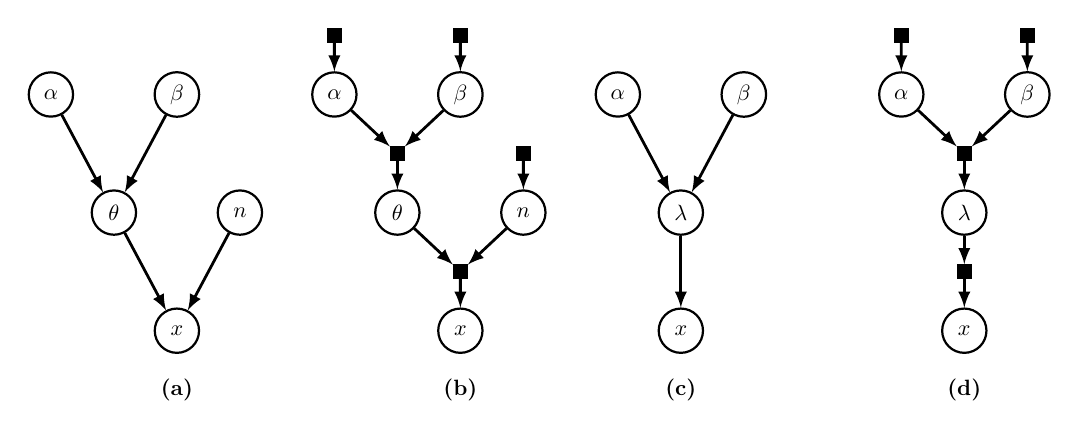
\begin{tikzpicture}[thick,xscale=0.8, yscale=.75, every node/.style={scale=0.8}]
\tikzset{vertex/.style = {shape=circle,draw,minimum size=2em}}
\tikzset{edge/.style = {->,> = latex, line width=1}}

% binomial beta directed graph
\begin{scope}
% vertices
\node[vertex] (a) at  (-1,2) {$\alpha$};
\node[vertex] (b) at  (1,2) {$\beta$};
\node[vertex] (x) at  (1, -2) {$x$};
\node[vertex] (n) at (2,0) {$n$};
\node[vertex] (t) at (0,0) {$\theta$};
%edges
\draw[edge] (a) to (t);
\draw[edge] (b) to (t);
\draw[edge] (t) to (x);
\draw[edge] (n) to (x);
\node at (1, -3) {\textbf{(a)}}; 
\end{scope}

% binomial beta factor graph
\begin{scope}[shift={(4.5,0)}]
% vertices
\node[vertex] (a) at  (-1,2) {$\alpha$};
\node[vertex] (b) at  (1,2) {$\beta$};
\node[vertex] (x) at  (1, -2) {$x$};
\node[vertex] (n) at (2,0) {$n$};
\node[vertex] (t) at (0,0) {$\theta$};
\begin{scope}[vertex/.style = {shape=rectangle, draw,minimum size=.1em, inner sep=3pt, fill=black}]
\node[vertex] (fone) at  (-1,3) {};
\node[vertex] (ftwo) at  (1,3) {};
\node[vertex] (fthree) at (0,1) {};
\node[vertex] (ffour) at (1,-1) {};
\node[vertex] (ffife) at (2,1) {};
\end{scope}
%edges

\draw[edge] (fone) to (a);
\draw[edge] (ftwo) to (b);
\draw[edge] (a) to (fthree);
\draw[edge] (b) to (fthree);
\draw[edge] (fthree) to (t);
\draw[edge] (t) to (ffour);
\draw[edge] (n) to (ffour);
\draw[edge] (ffour) to (x);
\draw[edge] (ffife) to (n);
\node at (1, -3) {\textbf{(b)}}; 
\end{scope}

% poisson gamma directed graph
\begin{scope}[shift={(9,0)}]
% vertices
\node[vertex] (a) at  (-1,2) {$\alpha$};
\node[vertex] (b) at  (1,2) {$\beta$};
\node[vertex] (l) at (0,0) {$\lambda$};
\node[vertex] (x) at (0,-2) {$x$};
%edges
\draw[edge] (a) to (l);
\draw[edge] (b) to (l);
\draw[edge] (l) to (x);
\node at (0, -3) {\textbf{(c)}}; 
\end{scope}

% poisson gamma factor graph
\begin{scope}[shift={(13.5,0)}]
% vertices
\node[vertex] (a) at  (-1,2) {$\alpha$};
\node[vertex] (b) at  (1,2) {$\beta$};
\node[vertex] (l) at (0,0) {$\lambda$};
\node[vertex] (x) at (0,-2) {$x$};
\begin{scope}[vertex/.style = {shape=rectangle, draw,minimum size=.1em, inner sep=3pt, fill=black}]
\node[vertex] (f1) at  (-1,3) {};
\node[vertex] (f2) at  (1,3) {};
\node[vertex] (f3) at  (0,1) {};
\node[vertex] (f4) at  (0,-1) {};
\end{scope}
%edges
\draw[edge] (f1) to (a);
\draw[edge] (f2) to (b);
\draw[edge] (a) to (f3);
\draw[edge] (b) to (f3);
\draw[edge] (f3) to (l);
\draw[edge] (l) to (f4);
\draw[edge] (f4) to (x);
\node at (0, -3) {\textbf{(d)}}; 
\end{scope}

\end{tikzpicture}


\caption{\label{fig:graphs_for_conj_priors}Directed graph (a) and factor graph (b) for beta distribution as conjugate prior of the binomial distribution. (c) and (d) shows the directed and factor graph for the Gamma distribution as conjugate prior of the Poisson distribution.}
\end{figure}
The structure of the underlying model is more transparent in a graph representation (Fig.\,\ref{fig:graphs_for_conj_priors} (a) and (b)). Apart from the Beta and Binomial distributions, there are the additional terms from the individual parameters. These terms eventually cancel in the computation for the conditional distribution,
\begin{align*}
p(\theta | \alpha, \beta, n, x)  &= \frac{p(\theta, \alpha, \beta, n, x)}{p(\alpha, \beta, n, x)} = \frac{p(\theta, \alpha, \beta, n, x)}{\int p(\theta, \alpha, \beta, n, x)\,d\theta} \\ &= \frac{p(x|n, \theta) p(\theta|\alpha, \beta)}{\int p(x|\theta, n) p(\theta|\alpha, \beta) \,d\theta},
\end{align*} 
which is just Equation \ref{eq:beta_binom} with the explicit form of the normalization constant.
\paragraph*{Example: Conjugate Prior for the Poisson distribution.} This example shows that the Gamma distribution is the conjugate prior to the Possion distribution. Assume the model for the data is a Poisson distribution,
\begin{align}
p(x|\lambda)= \frac{\lambda^x e^{-\lambda}}{x!},
\end{align}   
with $x$ number of counts. Chose the Gamma distribution $\Gamma(\lambda|\alpha, \beta)$  as Prior and assume only one Poisson experiment $x=(x)$ (see Fig.\,\ref{fig:graphs_for_conj_priors (c) and (d)}. Then we get as posterior
\begin{align}
p(\lambda|x, \alpha, \beta)  
&\propto  \frac{\lambda^x e^{-\lambda}}{x!} \Gamma(\lambda|\alpha, \beta) \\
&\propto \lambda^{(\alpha + x) - 1} e^{-\lambda(\beta +1)} \\
&\propto \Gamma(\lambda | \alpha + x, \beta +1)
\end{align} 
So, for one experiment $\alpha$ is updated by the number of counts  $x$  and $\beta$ is updated by the number of experiments (which is one). 

Now let's consider the case where we perform $n$ IID Poisson experiments, $x=(x_1, \dots, x_n)$. \textbf{(TODO graph with plate notation)} Then the likelihood becomes
\begin{align}
p(x|\lambda)= \prod _{i=1} ^n \frac{\lambda^{x_i} e^{-\lambda}}{x_i!}
=  \frac{\lambda^{\sum_{i=1}^n x_i} e^{-n \lambda}}{\prod _{i=1} ^n x_i!}
\end{align}
Then the posterior is obtained by
\begin{align}
p(\lambda|x, \alpha, \beta)  
&\propto  \frac{\lambda^x e^{-\lambda}}{x!} \Gamma(\lambda|\alpha, \beta) \\
&\propto  \lambda^{(\alpha + \sum_{i=1}^n x_i) - 1} e ^ {\lambda (\beta + n)} \\
&\propto \Gamma(\lambda | \alpha + \sum_{i=1}^n x_i, \beta +n)
\end{align}
So, for $n$ Poisson experiments the $\alpha$ parameter of the Gamma distribution is updated by the total number of counts (of all experiments) and beta is updated by the number of experiments ($n$ in this case).
\begin{theorem}
There exist conjugate priors for the exponential family of distributions.
\end{theorem}

%\section{Information Theory}
\paragraph*{Outlook.} This should also go into this section 
\begin{itemize}
\item definition of equivalent parametrization
\item Conditional Information
\item derivation of Jeffrey's prior
\item Flat vs Non-Informative Priors (high dimensional example)
\end{itemize}
 and $p$. \cite{barber}
 
\paragraph{Fisher information.}
\begin{definition}[Fisher information matrix] Assume that for the likelihood function $f(x|\theta)$, $\theta \in \mathbb{R}^n$ the FI regularity conditions hold \cite{schervish}. The Fisher information matrix is the covariance matrix with respect to the score function
\begin{align*}
I_{ij}(\theta) :=  \mathbb{E}_\theta \left[ \frac{\partial^2}{\partial \theta_i\partial \theta_j} \log f(x|\theta) \right], 
\end{align*}
where $\partial / \partial \theta_i \log f(x|\theta)$ is the $i$-th component of the score function. 
\end{definition} 
The fisher information depends on which of the several possible equivalent parametrizations is chosen. 

\begin{definition}[Jeffrey's Prior distribution] 
\begin{align*}
f(\theta) = c\, \sqrt{\det I},
\end{align*}
where $I$ is the Fisher information matrix and c is chosen such that $f(\theta)$ integrates to one if possible.  
\end{definition} 
If no such $c$ exists, then the  distribution $f(\theta)=\sqrt{\det I}$ is often used as improper prior distribution \cite{schervish}.
In the one dimensional case the fisher information becomes the second moment of the score function and Jeffreys prior is the square root of it. \textbf{Check: is the formular below really true (2nd derivative instead of square instead). }
\begin{align}
I(\theta)&=\mathbb{E}_\theta \left[\left( \frac{\partial \log f(x|\theta)}{\partial \theta}  \right) ^2\right] \\
f(\theta)&= c\, \sqrt{I}
\end{align} 

\paragraph{Example: Binomial distribution.}Suppose $X\sim Bin(n,p)$ given $P=p$ for a fixed $n$. Then, the Fisher information is obtained by
\begin{align*}
f_{X|P}(x|p) &=  \binom {n} {x} p^x (1-p)^{n-x}, \quad x=0,1,\dots, n \\
\partial_p(\log f_{X|P}(x|p)) &= \frac{x-np}{p(1-p)} \\
I(p) &= \frac{n}{p(1-p)},
\end{align*}
where we have used that the mean of the Binomial distribution is $np$ and that the variance of the Binomial distribution $\mathbb{E}\left[(x-\mu)^2\right] = np(1-p)$.
And Jeffrey's prior becomes,
\begin{align*}
f(p) \propto \sqrt{I} = n\, p^{-\frac{1}{2}}p^{-\frac{1}{2}} \propto Beta\left(1/2,1/2\right).
\end{align*}
Therefore, the $Beta(1/2, 1/2)$ distribution is a proper non-informative prior to the Binomial distribution. Note that the Beta distribution is also the conjugate prior to the Binomial distribution.

\paragraph*{Example: Poisson distribution.} Suppose $X\sim Poi(\lambda)$. The Fisher information is then 
\begin{align*}
f(x|\lambda) &= \frac{\lambda ^xe^{-\lambda}}{x!} \\
\partial_\lambda \log f(x|\lambda)  &=  \frac{x-\lambda}{\lambda} \\
I(\lambda) &= \frac{1}{\lambda^2}\mathbb{E}\left[(x-\lambda)^2\right] = \frac{1}{\lambda},
\end{align*}
where the formula for variance of the Poisson distribution, $\mathbb{E}\left[(x-\lambda)^2  \right] = \lambda$ was used. The Jeffrey's prior is thus,
\begin{align*}
f(\lambda) \propto \sqrt{I} = \lambda^{-\frac{1}{2}} \propto \Gamma(1/2, 0).
\end{align*}
This seems a bit odd because $\beta=0$ would lead to the constant zero for the $\Gamma$ distribution. However, since we are only interested in the proportionality, we can drop the $\beta^\alpha$ term in the Gamma distribution before setting the values. So, Jeffrey's Prior is an improper Gamma distribution. Improper because $\lambda^{-\frac{1}{1}}$ cannot be normalized. However, it is also of the same form as the conjugate prior. In real application it must be however ensured, that the posterior is a proper distribution. For this case this will be the case as soon as some observations have been made.

In summary the Jeffrey's prior is obtained be requiring invariance under a certain map on the likelihood. It is somewhat against the Baysian mind set where one first chooses a prior on the $\theta$ and then uses the likelihood in order to derive the posterior.

\paragraph{Kullback-Leibler divergence.} The Kullback-Leibler (KL) divergence measures the 'difference' between two distributions $q$ and $p$ \cite{barber}.This measure of information is designed to measure
how far apart two distributions are in the sense of likelihood. That is, if
an observation were to come from one of the distributions, how likely is
it that you could tell that the observation did not come from the other
distribution? \cite{schervish}
\begin{definition}[Kullback-Leibler Information]
\begin{align}
KL(q|p) := \langle \log \,q(x) - \log \,p (x)\rangle_{q(x)}  
\end{align}
\end{definition}
In general $KL(q|p) \geq 0$ and $KL(q|p) = 0   \Leftrightarrow q(x) = p(x)$ (in the sense that the respective probability measures have to be equal). However the KL is not a metric, because $KL(q|p) \neq KL(p|q)$. Even in the symmetrized case (which is sometimes itself called Kl divergence),  $KL(q|p) + KL(p|q)$, the triangle inequality does not hold. 

%\input{decision_theory.tex}
%\section{Linear models}

\paragraph{Interpretation}
\begin{itemize}
\item Predictive interpretation
\item Counterfacial interpretation
\end{itemize}
\paragraph{Interaction Terms}
\section{Generalized linear models}
%

\section{Classical distributions}

\paragraph*{Binomial distribution, $Bin(n,p)$.} Probability for the number of successes $x$ for $n$ IID bernoulli trials with chance of success $p$. The PMF is given by
\begin{align}
f(x|n,p) =  \binom {n} {x} p^x (1-p)^{n-x},
\end{align}
with mean $np$ and variance $np(1-p)$. \\

\paragraph*{Gamma distribution, $\Gamma(\alpha, \beta)$.} 
The $\Gamma$ has a rather generic form and contains the exponential distribution and chi-square distribution as special cases. In econometrics it is frequently used to model waiting times whereas in the Bayes framework it's mainly used as a conjugate prior for rate (inverse scale) parameters (occurring, e.g., in the Poisson or exponential distribution).
The PDF of the  Gamma distribution is defined as: $x\geq0$, $\alpha, \beta > 0$
\begin{align}\label{gamma_distri}
 f(x|\alpha,\beta) = 
 \frac{\beta^\alpha x^{\alpha -1} e^{-x\beta}}{\Gamma(\alpha)},
\end{align}
where $\Gamma(\alpha)$ is the \textbf{Gamma function}. It is the normalizing factor of the distribution to ensure that it integrates to one,
\begin{align}\label{gamma_function}
\Gamma(\alpha) = \int_0 ^\infty x^{\alpha -1} e^{-x}\, dx \\
\Gamma(\alpha + 1) = \alpha \Gamma(\alpha).
\end{align}
The Gamma function can be viewed as a generalization of the factorial to non-integer numbers. That for $n\in  \mathbb N, ~ \Gamma(n) = (n-1)!$ can be seen from the recursion formula. The recursion formula is in general very helpful. It can be derived by partial integration, 
$\partial_\alpha \Gamma(\alpha+1) = \int_0^\infty x^{\alpha}e^{-x}\, dx 
= -x^{\alpha}e^{-x}  \Big|_0^\infty +\alpha \int_0^\infty x^{\alpha-1}e^{-x}\,dx = 0 + \alpha\Gamma(\alpha)$.

Note that the Gamma function (\ref{gamma_function}) is indeed the normalization of the Gamma distribution (\ref{gamma_distri}). This can be seen by making the substitution $x\mapsto x\beta$ in the integration of Equation (\ref{gamma_distri}).

\paragraph*{Beta distribution, $Beta(\alpha, \beta)$.} Is used to model distributions over probabilities because it has a very flexible form. The Beta distribution has the domain of definition $\alpha, \beta > 0, \theta \in [0,1]$ (some authors have the open interval for theta). The pdf is defined as.
\begin{align}
f(x|\alpha, \beta) = \frac{1}{B(\alpha, \beta)}x^{\alpha-1}(1-x)^{\beta-1}
\end{align} 
where $B$ is the \textbf{Beta function}. It just normalizes the Beta distribution and it is often more convenient to express it via the $\Gamma$ function.
\begin{align}
B(\alpha, \beta) = \int_0^1 x^{\alpha-1}(1-x)^{\beta-1}\,dx = \frac{\Gamma(\alpha) \Gamma(\beta)}{\Gamma(\alpha + \beta)}
\end{align}
The beta distribution has mean \footnote{To see the mean, we evalute the k-th moment $E(x^k) =  \frac{1}{B(\alpha, \beta)}\int x^{\alpha-1 + k}(1-x)^{\beta-1} dx$. Multiplying and dividing by $B(\alpha+k, \beta)$ the integrand gets one and we get $E(x^k) = \frac{B(\alpha+k, \beta)}{B(\alpha+k, \beta)}$ The mean is given for $k=1$. Rewriting in terms of the $\Gamma$ function  we get, $E(x) = \frac{\Gamma(\alpha + \beta)}{\Gamma(\alpha) \Gamma(\beta)} \frac{\Gamma(\alpha + 1) \Gamma(\beta)}{\Gamma(\alpha+\beta+1)} = \frac{\alpha}{\alpha+\beta}$} 
$\frac{\alpha}{\alpha + \beta}$ and variance $\frac{\alpha \beta}{(\alpha+\beta)^2 (\alpha+\beta+1)} $. For $\alpha, \beta > 1$ the maximum is given by $\frac{\alpha-1}{\alpha+\beta -2}$. 

\paragraph*{Poisson distribution,} $Poi(\lambda)$. Is used to model  the number of events $k$ ('counts') in a fixed (time) interval. The pmf is defined as 
\begin{align}
f(k|\lambda) = \frac{\lambda^k e^{-\lambda}}{k!}, \quad k\in \mathbb{N}, \lambda \in \mathbb{R}_{>0},
\end{align} 
where $\lambda$ is the event rate or rate parameter. It describes the expected number of events per interval (indeed it is also the expectation value of the Poisson distribution).

\subsubsection*{Multivariate Normal distribution}
\begin{align}
\mathcal{N}(\mu, \Sigma) &= p(x|\mu, \Sigma) \\ 
 &= -\frac{1}{\sqrt{\det(2\pi\Sigma)}}e^{-\frac{1}{2}(x-\mu)^\intercal \Sigma^{-1} (x-\mu)},
\end{align}
with mean vector $\mu$, covariance matrix $\Sigma$ and its inverse the  precision matrix $\Sigma^{-1}$.
It can be shown that,
\begin{align}
\mu &= \langle x \rangle_{\mathcal{N}(\mu, \Sigma)} \\ 
\Sigma &= \langle (x-\mu) (x-\mu)^ \intercal ) \rangle_{\mathcal{N}(\mu, \Sigma)} \\ 
\end{align}

\paragraph*{Transformations}
\begin{itemize}
\item $y=Ax$
\end{itemize}
Let $x\sim \mathcal{N}(\mu, \Sigma)$ and $A$ be a regular  Matrix (i.e, non-singular, $\det(A)\neq 0 $). Then under the  transformtion $y=Ax$,  $y$ is again normally distributed, $y \sim \mathcal{N}(A\mu, A\Sigma A^\intercal)$.
\begin{proof}
Using the transformation law with jacobian $\det(A)$ gives 
\begin{align*}
f_Y(y) &= \frac{f_X(A^{-1}y)}{\det(A)} \\
&= \frac{1}{\det(A) \sqrt{2\pi\Sigma}} e^{-\frac{1}{2} (A^{-1}y-\mu)^\intercal \Sigma^{-1} (A^{-1}y-\mu)} \\
&=  \frac{1}{\sqrt{2\pi\Sigma_y}} e^{-\frac{1}{2} (y-A\mu)^\intercal \Sigma_y^{-1} (y-A\mu)},
\end{align*}
where we have used $\mu = 1 \mu = A^{-1} A \mu$ and identified $\Sigma_y^{-1} = A ^{-1\intercal} \Sigma^{-1} A^{-1}$ and therefore $\Sigma_y = A \Sigma A^\intercal$ 

\end{proof}
\begin{itemize}
\item $z=x + y$
\end{itemize}
Let $x\sim \mathcal{N}(\mu_x, \Sigma_x)$ and $y\sim \mathcal{N}(\mu_y, \Sigma_y)$ be two independent Normal distributions $x$. Then $z=x+y$ is again normally distributed with $z \sim \mathcal{N}(\mu_x + \mu_y, \Sigma_x + \Sigma_y)$


\begin{proof}
By Theorem \ref{thm:sum_rv} we have for the pdf
\begin{align}
&f_{X+Y}(z) 
= f_X(x) \star f_Y(y) = \int f_X(z - y)f_Y(y)\,dy  \\
&= \frac{1}{\sqrt{\det (2\pi \Sigma_x)}\sqrt{\det (2\pi \Sigma_y)}} \int  e ^ {-\frac{1}{2}\left[(z-y-\mu_x)^\intercal \Sigma_x^{-1} (z-y-\mu_x)+ (y - \mu_y)^\intercal\Sigma_y^{-1} (y - \mu_y)\right]} \,dy
\label{eq:sum_normal_intermediate0}
\end{align}
We focus on the square bracket in the exponent, define the quantities $\bar y = y - \mu_y$, $\bar z = z - \mu_x - \mu_y$, and proceed by completing the square with respect to $y$.
\begin{align}
[\cdot] 
&= \bar y^\intercal\Sigma_y^{-1} \bar y + (\bar y - \bar z )^\intercal\Sigma_x^{-1} (\bar y - \bar z) \\
&= \bar y^\intercal(\Sigma_y ^{-1} + \Sigma_x ^{-1}) \bar y  - 2 {\bar z} ^ \intercal\Sigma_x ^{-1} \bar y + \bar z^\intercal  \Sigma_x ^{-1} \bar z  \label{eq:sum_normal_intermediate1}
\end{align}
In order to complete the squere, note that both $\Sigma$ are symmetric and invertible. Therefore, also the inverse is symmetric and their (inverse) sum is symmetric and invertible. Now, set $\tilde \Sigma ^{-1}:= \Sigma_y ^{-1} + \Sigma_x ^{-1}$ and consider the term 
\begin{align*}
(\bar y - \tilde \Sigma \Sigma_x^{-1}\bar z)^\intercal \tilde \Sigma ^{-1} (\bar y - \tilde \Sigma \Sigma_x^{-1}\bar z) 
= \bar y ^\intercal \tilde \Sigma ^{-1} \bar y 
- 2  {\bar z} ^ \intercal\Sigma_x ^{-1} \bar y
+ \bar z^\intercal \Sigma_x^{-1} \tilde \Sigma  \Sigma_x^{-1} \bar z
\end{align*}
Rearranging this identity and plugging it into expression (\ref{eq:sum_normal_intermediate1}), gives
\begin{align}
[\cdot] & = (\bar y - \tilde \Sigma \Sigma_x^{-1}\bar z)^\intercal \tilde \Sigma ^{-1} (\bar y - \tilde \Sigma \Sigma_x^{-1}\bar z) - \bar z^\intercal \Sigma_x^{-1} \tilde \Sigma  \Sigma_x^{-1} \bar z  + \bar z^\intercal  \Sigma_x ^{-1} \bar z \label{eq_matrix_normal_2}\\ 
&= (\bar y - \tilde \Sigma \Sigma_x^{-1}\bar z)^\intercal \tilde \Sigma ^{-1} (\bar y - \tilde \Sigma \Sigma_x^{-1}\bar z) + \bar z^\intercal (\Sigma_x + \Sigma_y)^{-1} \bar z,
\end{align}
where in the last step the useful Matrix identities\footnote{Let $X, Y$ be regualar matrices. Then:
\begin{align} \label{eq:matrix_id_1}
X^{-1}(X^{-1} + Y^{-1})^{-1}Y^{-1} = (X+Y)^{-1}.
\end{align}
Set the left hand side $Z:=X^{-1}(X^{-1} + Y^{-1})^{-1}Y^{-1}$. Its inverse is apparently $Z^{-1} =  X + Y$ Therefore,  $Z =  (X + Y)^{-1}$. The second matrix identity reads
\begin{align} 
X^{-1}  - X^{-1}(X^{-1} + Y^{-1})^{-1}X^{-1} = (X+Y)^{-1}.
\end{align}
The left hand side can be rewritten as $X^{-1}  - X^{-1}(X^{-1} + Y^{-1})^{-1}(X^{-1}\pm Y^{-1}) = X^{-1}(X^{-1} + Y^{-1})^{-1}Y^{-1} = (X+Y)^{-1 }$, where in the last step identity (\ref{eq:matrix_id_1}) was used.} were used. We can now plug this expression back into (\ref{eq:sum_normal_intermediate0}). Unter the integral the first term evaluates to $\sqrt{\det(2\pi\tilde\Sigma)}, \forall \bar z$. Taking into account that $\det\tilde \Sigma /  (\det\Sigma_x\det  \Sigma_y) = 1 / \det(\Sigma_x(\Sigma_x^{-1}+\Sigma_y^{-1})\Sigma_y) = 1/\det(\Sigma_x+\Sigma_y)$ eventually gives 
\begin{align}
 (\ref{eq:sum_normal_intermediate0})  
 &= 
 \frac{\sqrt{\det(2\pi\tilde\Sigma)}}{\sqrt{\det(2\pi\Sigma_x)\det(2\pi\Sigma_x)}} 
  e^{-\frac{1}{2} (z-\mu_x - \mu_y)^\intercal (\Sigma_x + \Sigma_y)^{-1}(z-\mu_x - \mu_y) } \\ 
  &=\frac{1}{\sqrt{\det(2\pi(\Sigma_x+\Sigma_y))}} e^{-\frac{1}{2} (z-\mu_x - \mu_y)^\intercal (\Sigma_x + \Sigma_y)^{-1}(z-\mu_x - \mu_y) }  \\
  &= \mathcal{N}(\mu_x + \mu_y, \Sigma_x + \Sigma_y)
\end{align}
\end{proof}
\paragraph*{Remark} 
A somewhat less matrix-magic approach ist to pause the computation at equation (\ref{eq_matrix_normal_2}) and realizing that this already establishes a quadratic form in $\bar z$ and thus a normal distribution in $z$. In order to get the expressions vor $\mu_z$ and $\Sigma_z$ one could alternatively calculate them by using the linearity property of the expectation value together with the independence assumption $f_{X,Y}(x,y)=f_X(x)f_Y(y)$:
\begin{align}
\mu_z = \langle z \rangle =\iint f_X(x)f_Y(y) (x+y)\, dx\,dy =\langle x \rangle + \langle y \rangle  = \mu_x + \mu_y
\end{align}
\begin{align}
\Sigma_z &= \langle(x+y-\mu_x - \mu_y)(x+y-\mu_x - \mu_y)^\intercal\rangle  \\ 
&= \langle (x-\mu_x)(x - \mu_x)^\intercal \rangle +  \langle (y-\mu_y)(y - \mu_y)^\intercal \rangle + 2\langle (x-\mu_x)(y - \mu_y)^\intercal \rangle  \\
&= \langle (x-\mu_x)(x - \mu_x)^\intercal \rangle +  \langle (y-\mu_y)(y - \mu_y)^\intercal \rangle,
\end{align}
where the symmetry of $\Sigma$ was used (factor 2) and the last term vanishes because of independence ($\iint f_X(x)f_Y(y) (x-\mu_x)(x-\mu_x)^\intercal = 0$).
\begin{itemize}
\item $z=Ax + y$
\end{itemize}
Let $x\sim \mathcal{N}(\mu_x, \Sigma_x)$ and $y\sim \mathcal{N}(\mu_y, \Sigma_y)$ be two independent Normal distributions $x$. Then $z=Ax+y$  with $A$ being a regular matrix is again normally distributed with $z \sim \mathcal{N}(A\mu_x + \mu_y,  A\Sigma_xA^\intercal+\Sigma_x)$

\begin{proof}
This follows immeadiatly by composition of the above results. Set $\tilde x =  Ax$. Then $z = \tilde x + y \sim \mathcal{N}(\mu_{\tilde{x}} + \mu_y, \Sigma_{\tilde{x}} + \Sigma_y ) = \mathcal{N} (A\mu_{x} + \mu_y, A \Sigma_{x} A^\intercal + \Sigma_y ) $
\end{proof}
\bibliography{papers}
\end{document}
